\section{2D 2G Quarter Core}
This problem is a more traditional $k$-eigenvalue criticality problem using neutron diffusion.  We simulate a benchmark reactor core by imposing reflecting conditions on the left and bottom boundaries of a quarter-core geometry.  The governing PDE for this equation is still
\begin{equation}
-\drv{}{x}D_g\drv{\phi_g}{x}+(\Sigma_{g,a}+\Sigma_{g,s})\phi_g = \sum_{g'}\sigma_{s}^{g'\to g}\phi_{g'} + \frac{\chi_{g}}{k}\sum_{g'}\nu_{g'}\sigma_{f,g'}\phi_{g'},\hspace{15pt} g\in[1,2],
\end{equation}
where $g$ denotes the energy group, $D$ is the group diffusion cross section; $\phi$ is the group flux, $x$ is the location within the problem; $\Sigma_a,\Sigma_s,\Sigma_f$ are the macroscopic absorption, scattering, and fission cross sections respectively; $k$ is the criticality factor eigenvalue and quantity of interest; and $\chi$ is the fraction of neutrons born into an energy group.  In this case, we consider only downscattering, and fission neutrons are only born into the high energy group ($\Sigma_s^{2\to1}=\chi_2=0$).

This problem also does not have a convenient general analytic solution.  We can express the solver as
\begin{equation}
U(p;\theta) = k(p;\Sigma_{2,a}),
\end{equation}
where
\begin{equation}
p=(D_g,\Sigma_{1,a},\Sigma_{g,s},\nu_g,\Sigma_{g,f},\chi_g),\hspace{20pt}g\in[1,2].
\end{equation}
While $\phi_g(x)$ might also be considered a parameter, it is an output value solved simultaneously with $k$.

For this test code we consider $\theta=\Sigma_{2,a}$ normally distributed as $\theta\in\mathcal{N}(0.1003,0.0001)$. Tabular data for mean and variance convergence is in Table \ref{tab:2dcrit}, and the pdfs obtained are in Fig. \ref{fig:2dcrit}.  Once again, it is important to note that the Monte Carlo sampling was restricted to values within 3 standard deviations of the mean; as such, the means and variances obtained directly through Monte Carlo sampling are not representative of the full uncertainty space.  This truncation of the distribution is enforced because without such a restriction, it is possible to sample physically untenable values for $\Sigma_{2,a}$, including negative values.

\begin{table}
\begin{center}
\begin{tabular}{c c|l l}
type & runs/order & mean & variance \\ \hline
MC & $1\times10^6$ & 1.01488024214 & 0.00196794483094 \\
SC & 2 & 1.01617227356 & 0.00103920580302 \\
SC & 4 & 1.01543109812 & 0.0020042932657 \\
SC & 8 & 1.015592044 & 0.00192541919329 \\
SC & 16 & 1.01549506606 & 0.00189209311817 \\
SC & 32 & 1.01061893249 & 0.00227815756915
\end{tabular}
\end{center}
\caption{Convergence of Mean, Variance for 2D2G Case}
\label{tab:2dcrit}
\end{table}

\begin{figure}[h!]
\centering
   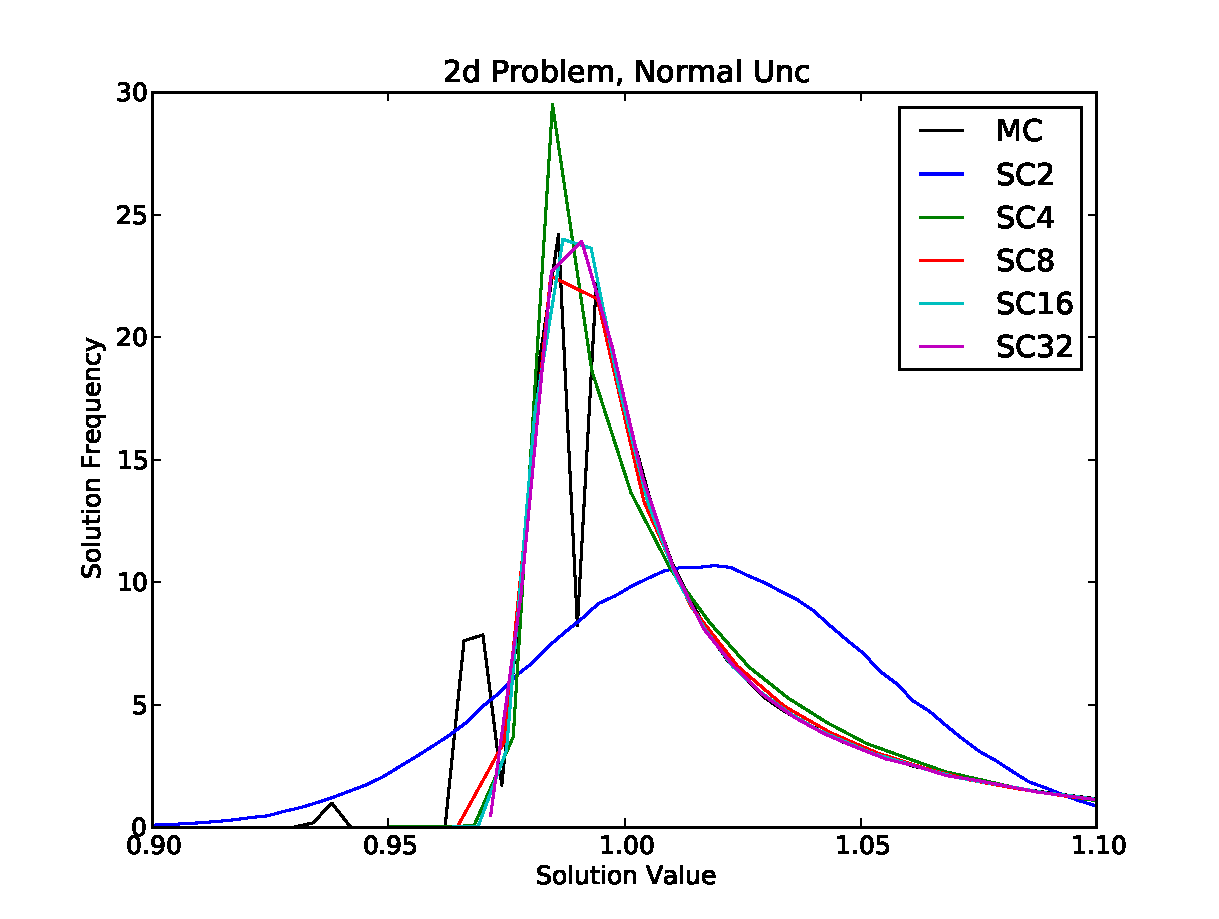
\includegraphics[width=\textwidth]{../graphics/2d_normal_pdfs}
   \caption{Solution PDF Convergence, 2D2G Case}
   \label{fig:2dcrit}
\end{figure}


%
%\begin{figure}[h!]
%\centering
%   \includegraphics[width=\textwidth]{../graphics/}
%   \label{}
%   \caption{}
%\end{figure}
%\begin{table}
%\begin{center}
%\begin{tabular}{c c|l l| r}
%type & runs/order & mean & variance & run time (sec) \\ \hline
%MC & 1\times10^6 &  &  & \\
%SC & 2 & & & \\
%SC & 4 & & & \\
%SC & 8 & & & \\
%SC & 16 & & &
%\end{tabular}
%\end{center}
%\caption{}
%\label{}
%\end{table}
%
%\begin{figure}[h!]
%\centering
%   \includegraphics[width=\textwidth]{../graphics/}
%   \label{}
%   \caption{}
%\end{figure}
